\documentclass[a4paper]{article}

\usepackage[T1]{fontenc}
% many useful symbols
\usepackage{textcomp}
\usepackage[italian]{babel}
\usepackage{hyperref}
\usepackage{amsmath, amssymb, amsthm}
\usepackage{mathtools}
% for \lightning
\usepackage{stmaryrd}
\usepackage{geometry}
\usepackage{tikz-cd}
\usepackage{cancel}

% Remove indentation globally
\setlength{\parindent}{0pt}
% Have blank lines between paragraphs
\usepackage[parfill]{parskip}

\hypersetup{
    colorlinks = true, % links instead of boxes
    urlcolor   = cyan, % external hyperlinks
    linkcolor  = blue, % internal links
    citecolor  = cyan   % citations
}

\newcommand{\R}{\mathbb{R}}
\newcommand{\C}{\mathbb{C}}
\newcommand{\Q}{\mathbb{Q}}
\newcommand{\N}{\mathbb{N}}
\newcommand{\A}{\mathbb{A}}
\newcommand{\Z}{\mathbb{Z}}

% use bullets for items
\renewcommand{\labelitemii}{$\circ$}

\newcommand{\im}{\operatorname{im}}
\newcommand{\coker}{\operatorname{coker}}

\newcommand\numberthis{\addtocounter{equation}{1}\tag{\theequation}}

% Display math
\newcommand{\ssfrac}[2]{
	\raisebox{+0.3ex}{$#1$}
	/
	\raisebox{-0.3ex}{$#2$}
}
% Inline math
\newcommand{\sfrac}[2]{
	\raisebox{+0.3ex}{\scalebox{0.9}{$#1$}}
	/
	\raisebox{-0.3ex}{\scalebox{0.9}{$#2$}}
}

 % No white line in equal arrows
\usetikzlibrary{decorations.markings}
\tikzset{double line with arrow/.style args={#1,#2}{decorate,decoration={markings,%
                    mark=at position 0 with {\coordinate (ta-base-1) at (0,1pt);
                            \coordinate (ta-base-2) at (0,-1pt);},
                    mark=at position 1 with {\draw[#1] (ta-base-1) -- (0,1pt);
                            \draw[#2] (ta-base-2) -- (0,-1pt);
                        }}}}
\tikzset{Equal/.style={-,double line with arrow={-,-}}}


\newtheorem{theorem}{Theorem}[section]
\newtheorem{lemma}[theorem]{Lemma}

\theoremstyle{definition}
\newtheorem{definition}[theorem]{Definition}

\theoremstyle{definition}
\newtheorem{example}[theorem]{Example}

\theoremstyle{remark}
\newtheorem*{remark}{Remark}

\theoremstyle{definition}
\newtheorem{exercise}{Esercizio}[section]
\newtheorem*{exercise*}{Esercizio}

\title{Elementi di Topologia Algebrica - Gruppo 1}

\begin{document}
\maketitle

\textbf{Esercizio 1}
Costruiamo la realizzazione geometrica di $\Delta$ dentro $\R^N$, dove $N=|\Delta|$: ordinati gli elementi $\{x_1,\ldots,x_N\}$ di $X$ contenuti
nelle facce di $\Delta$ (in altre parole, i suoi vertici), e se $\tau=\{x_{i_0},\ldots,x_{i_k}\}$ è una faccia di dimensione $k$ poniamo
\[
    X(\tau) = \im(\varphi: \Delta^{k} \to \R^N),
\]
dove $\varphi$ è la mappa lineare definita da
\[
    \varphi(e_j) = e_{i_j}
\]
per $j=0,\ldots,k$. La realizzazione geometrica di $\Delta$ è quindi l'insieme
\[
    X(\Delta) \coloneqq \bigcup_{\tau \in \Delta} X(\tau).
\]
Inoltre, se $\tau,\tau^\prime \in \Delta$,
\[
    X(\tau \cap \tau^\prime) = \left\{ \sum_{x_i \in \tau \cap \tau^\prime} \lambda_i e_i \mid \lambda_i\geq 0,~ \sum_{x_i \in \tau \cap \tau^\prime} \lambda_i = 1 \right\}
\]
    \[= \left\{ \sum_{x_i \in \tau } \lambda_i e_i \mid  \lambda_i\geq 0,~\sum_{x_i \in \tau } \lambda_i = 1 \right\} \cap \left\{ \sum_{x_i \in \tau^\prime } \lambda_i e_i \mid \lambda_i\geq 0,~\sum_{x_i \in \tau^\prime} \lambda_i = 1
    \right\} = X(\tau) \cap X(\tau^\prime).
\]

\textbf{Esercizio 2}
Dimostriamo innanzitutto che il complesso di catene $$C_\bullet\coloneqq C_\bullet(\mathcal{P}{([n])})$$ è esatto, da cui seguirà che questo ha omologia ridotta nulla, ovvero $\widetilde{H}_k(\mathcal{P}{([n])}) =
0$ per ogni $k$. Per fare ciò, costruiamo un'omotopia di catene tra l'identità e la mappa nulla da $C_\bullet$ in sé: fissato $k$, definiamo tale omotopia di catene sulla base di $C_k$ come $\Z$-modulo libero data dai $k$-simplessi:
\[
    s_k: C_k \to C_{k+1},\qquad s_k(\tau) =
    \begin{cases}
        0 & \text{se } 0 \in \tau \\
         \tau \cup\{0\} & \text{altrimenti}
    \end{cases}
\]
Verifichiamo la relazione
\[
    \partial s + s\partial = \operatorname{id}
:\]
\begin{itemize}
    \item se $0 \in \tau$, allora $\partial s(\tau) = \partial(0) = 0,$ e inoltre
        \[
            s \partial (\tau) = s \left(\sum_{x\in \tau} (-1)^{|\{x^\prime < x\}|} \tau\setminus\{x\} \right) = \tau + s \left(\sum_{x\in \tau,x\neq 0} (-1)^{|\{
                x^\prime < x\}|} \underbrace{\tau\setminus\{x\}}_{\text{contiene 0}} \right) = \tau
        .\]
    \item se $0 \notin \tau$, allora
        \begin{align*}
           &\partial s(\tau) + s\partial(\tau) \\
           &= \partial(\tau \cup \{0\}) + s\left(\sum_{x\in \tau} (-1)^{|\{x^\prime < x\}|} \tau\setminus\{x\}\right) \\
           &= \tau + \sum_{x\in \tau} (-1)^{|\{x^\prime < x,~x^\prime\in\tau\cup\{0\}\}|} (\tau\cup\{0\})\setminus\{x\} + \sum_{x\in \tau} (-1)^{|\{x^\prime < x,~x^\prime\in\tau\}|} (\tau\cup\{0\})\setminus\{x\} \\
            &= \tau.
    \end{align*}
\end{itemize}

    Se poi chiamiamo $D_\bullet$ il complesso di catene associato a $\Delta^n=\mathcal{P}{([n])}\setminus \{[n]\}$, osserviamo che $D_k=C_k\simeq \Z^{\binom{n+1}{k+1}}$ per ogni
    $k<n$ in quanto le facce di tali dimensioni coincidono, e che quindi
    \[
        \widetilde{H}_k(\Delta^n) = \widetilde{H}_k(\mathcal{P}([n])) = 0
    \]
    per ogni $k<n-1$; inoltre, $D_{n}=0$ perché abbiamo rimosso l'unica faccia di dimensione $n$, quindi $\widetilde{H}_n(\Delta^n) = 0$.

    Infine, per calcolare $\widetilde{H}_{n-1}(\Delta^n)$, consideriamo il seguente diagramma (commutativo per l'omotopia costruita sopra):
    \[
        \begin{tikzcd}
            0 \arrow[r] & C_{n} \arrow[r,"\partial_n"] \arrow[d] & C_{n-1} \arrow[r] \arrow[d, Equal] & C_{n-2} \arrow[d,Equal]  \\
                        & D_n \arrow[r] & D_{n-1} \arrow[r,"\partial_{n-1}"] & D_{n-2}
        \end{tikzcd}
    \]
    Visto che $D_{n}=0$, si ha
    \[
        \widetilde{H}_{n-1}(\Delta^n) = \ker(\partial_{n-1}) = \im(\partial_n) = C_n \simeq \Z
    .\]
    Avendo calcolato l'omologia ridotta di $\Delta^n$, concludiamo che
    \[
        H_k(\Delta^n) =
        \begin{cases}
             \Z & \text{se } k=0,n-1\\
             0 & \text{altrimenti}
        \end{cases}
    \]


\textbf{Esercizio 3}
Vogliamo dimostrare la commutatività del diagramma

\begin{center}
    \begin{tikzcd}
        \pi_1(X) \arrow[d, "h_X"] \arrow[r, "f_\#"] & \pi_1(X) \arrow[d, "h_Y"] \\
        H_1(X) \arrow[r, "f_\ast"] & H_1(Y)
    \end{tikzcd}
\end{center}
Ricordandoci che la mappa $h_X$ manda la classe di un loop $\gamma$ nella classe del ciclo $c_\gamma$ definito da
\[
    c_\gamma(t,1-t) = \gamma(t),
\]
abbiamo che
\[
    h_Y(f_\#([\gamma])) = h_Y([f\circ \gamma]) = [c_{f\circ \gamma}] = [f\circ c_\gamma] = f_* \circ h_X([\gamma]),
\]
dove la penultima uguaglianza segue osservando che entrambi i cicli $c_{f\circ \gamma}$ e $f\circ c_\gamma$ mandano
$(t,1-t)$ in $f(\gamma(t))$.

\textbf{Esercizio 4} Visto che $S^1\times S^1$ è connesso per archi, abbiamo che
\[
    H_0(S^1\times S^1) = \Z,\qquad H_1(S^1\times S^1) \simeq \pi_1(S^1\times S^1)^{ab} = \Z^2
.\]

Prendiamo ora un ricoprimento di $S^1\times S^1$ dato da due cilindri $A$ e $B$, che si intersecano a loro volta in due cilindri disgiunti. Ciascuno di tali cilindri è omotopicamente
equivalente a $S^1$, e sappiamo che
\[
    H_n(S^1) = \begin{cases}
        \Z & \text{se } n=0,1 \\
        0 & \text{altrimenti}
    \end{cases}
.\]
Inoltre, visto che l'omologia è additiva rispetto all'unione disgiunta, l'omologia di $A\cap B$ è la somma diretta delle omologie di $A$ e $B$, ed quindi in grado n è la somma diretta di due
copie di $H_n(S^1)$.

La successione di Mayer-Vietoris ci dà quindi la seguente successione esatta per $n\geq 3$:
\[
    \ldots\to \cancel{H_n(A\cap B)} \to \cancel{H_n(A) \oplus H_n(B)} \to H_n(S^1\times S^1) \to \cancel{H_{n-1}(A\cap B)} \to \ldots,
\]
da cui otteniamo che $H_n(S^1\times S^1) = 0$ per $n\geq 3$.
Resta quindi il caso $n=2$, per il quale la successione è
\[
    0 \to H_2(S^1\times S^1) \overset{\alpha}{\to} H_1(A\cap B) \overset{\beta}{\to} H_1(A) \oplus H_1(B) \to \ldots,
\]
ovvero a meno di isomorfismo
\[
    0 \to H_2(S^1\times S^1) \to \Z^2 \to \Z^2 \to \ldots,
\]
ed essendo $\alpha$ iniettiva, per esattezza otteniamo che $H_2(S^1\times S^1)$ è isomorfo al kernel di $\beta$.

D'altronde, presi dei generatori $a$ e $b$ dell'omologia dell'intersezione, osserviamo che visti in $A$ ed in $B$ questi generano $H_1(A)$ e $H_1(B)$ rispettivamente, e quindi sono
omologhi. In altre parole, $\beta(a)=\beta(b) = c$ per qualche $c\in H_1(A)\oplus H_1(B)$ che corrisponde all'elemento $(1,1)\in \Z^2$, quindi l'immagine di $\beta$ è isomorfa a $\Z$.
In conclusione, $H_2(S^1\times S^1) \simeq \ker(\beta) $ è isomorfo a $\Z$, in quanto il kernel è generato da $a-b$.

\newpage
\textbf{Esercizio 5}

Il complesso simpliciale astratto $\Delta$ che useremo è descritto dalla seguente disegno (dove i vertici con lo stesso indice sono identificati), la cui realizzazione geometrica risulta omeomorfo al toro:

\begin{center}
    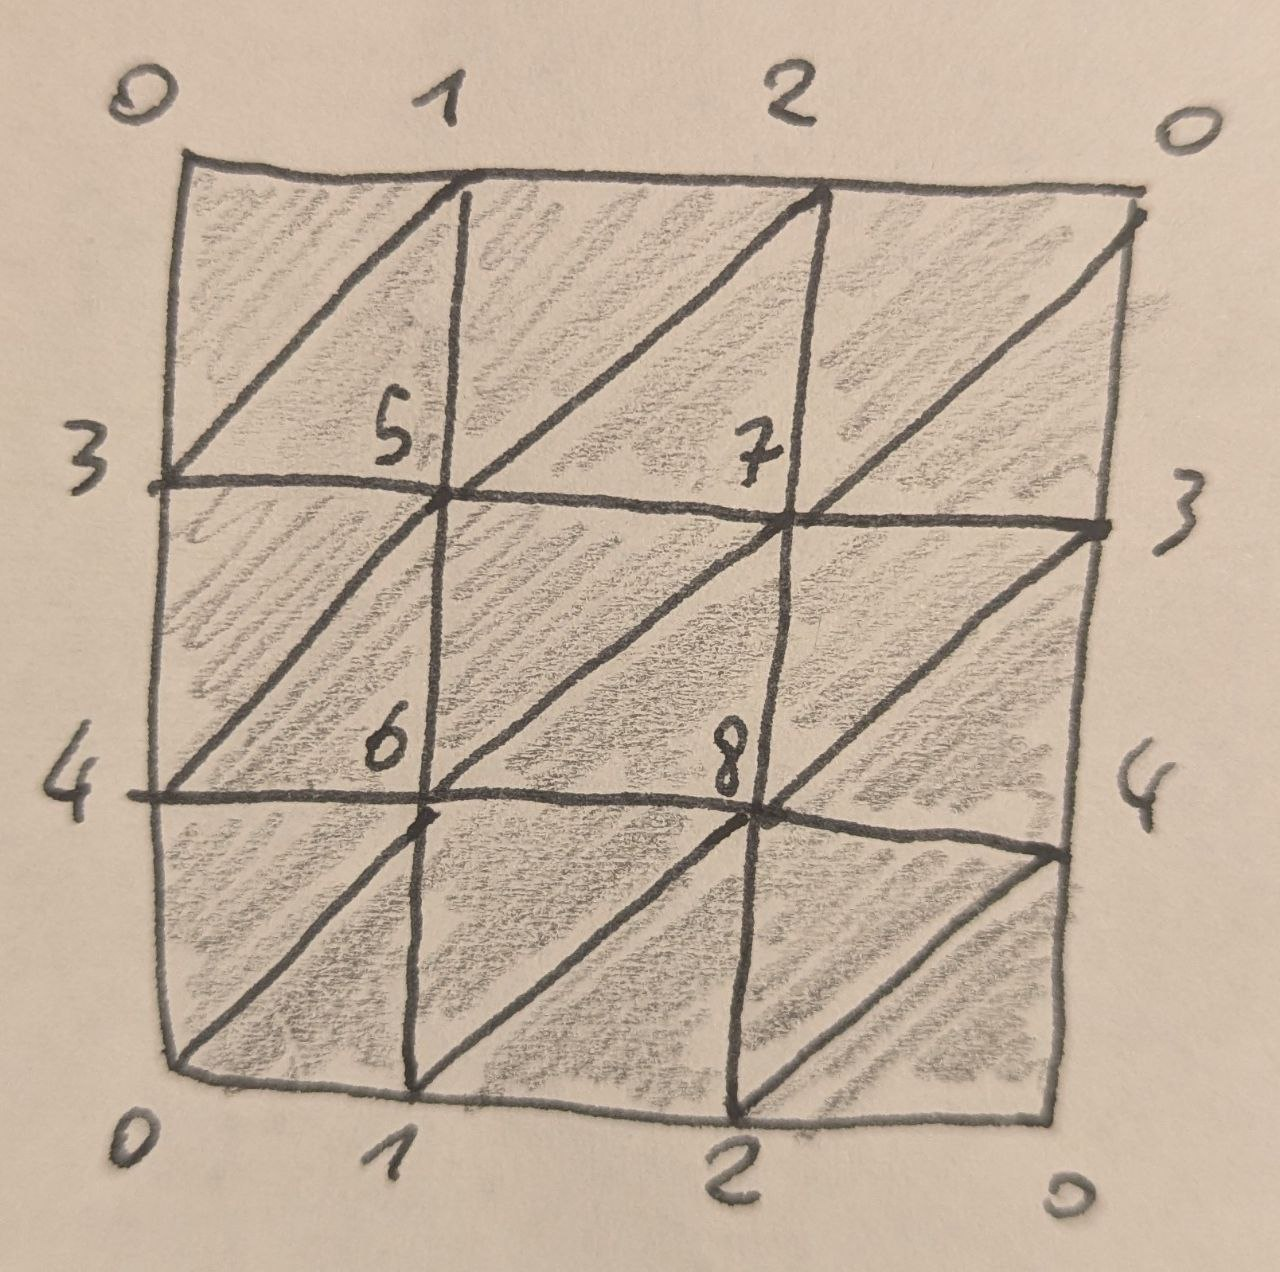
\includegraphics[width=0.5\textwidth]{toro.jpg}
\end{center}

Il complesso di catene associato a $\Delta$ è

\[
\ldots \to 0 \to C_2 \overset{\partial_2}{\to} C_1 \overset{\partial_1}{\to} C_0 \to 0 \to \ldots
,\]
dove contando i simplessi dopo aver identificato i vertici, si ha che $C_0 \simeq \Z^9$, $C_1 \simeq \Z^{27}$ e $C_2 \simeq \Z^{18}$.

Calcoliamone l'omologia: $H_0(\Delta) = \sfrac{C_0}{\im(\partial_1)}$, e visto che $\partial_1$ manda un 1-simplesso nella differenza fra i suoi vertici, nel quoziente stiamo
identificando tutti i vertici nella stessa componente connessa all'interno del grafo associato a $\Delta$, ma questi sono tutti i vertici; questo mostra che $H_0(\Delta)\simeq\Z$.

Inoltre sappiamo che $H_2(\Delta)=\ker(\partial_2)$, e dato $\tau=\{a,b,c\}$ un 2-simplesso con $a<b<c$ questo ha bordo
\[\partial_2(\tau)=\{b,c\}-\{a,c\}+\{a,b\},\] e si vede facilmente che
le uniche combinazione di
tali simplessi che danno $0$ sono i multipli della somma di \textit{tutti} i triangoli (sommare i bordi di due triangoli adiacenti ha l'effetto di cancellare la faccia in comune), per cui
$H_2(\Delta) \simeq \Z$.

Infine, osserviamo che dai conti svolti sopra e dal primo teorema di isomorfismo otteniamo
\[
\begin{cases}
    \im(\partial_2) \simeq \sfrac{C_2}{\ker(\partial_2)} \simeq \sfrac{\Z^{18}}{\Z} = \Z^{17} \\
    \im(\partial_1) \simeq \sfrac{C_1}{\ker(\partial_1)}\simeq \sfrac{\Z^{27}}{\ker(\partial_1)} \overset{\im(\partial_1)\simeq\Z^8 }{\implies} \ker(\partial_1) \simeq \Z^{19},
\end{cases}
\]

dove l'ultima implicazione segue dal fatto che tutti i gruppi coinvolti sono $\Z$-moduli liberi, e quindi
\[
    H_1(\Delta)=\ssfrac{\ker(\partial_1)}{\im(\partial_2)} \simeq \ssfrac{\Z^{19}}{\Z^{17}} = \Z^2
.\]

\end{document}
